\documentclass[twoside]{book}

% Packages required by doxygen
\usepackage{calc}
\usepackage{doxygen}
\usepackage{graphicx}
\usepackage[utf8]{inputenc}
\usepackage{makeidx}
\usepackage{multicol}
\usepackage{multirow}
\usepackage{textcomp}
\usepackage[table]{xcolor}

% Font selection
\usepackage[T1]{fontenc}
\usepackage{mathptmx}
\usepackage[scaled=.90]{helvet}
\usepackage{courier}
\usepackage{amssymb}
\usepackage{sectsty}
\renewcommand{\familydefault}{\sfdefault}
\allsectionsfont{%
  \fontseries{bc}\selectfont%
  \color{darkgray}%
}
\renewcommand{\DoxyLabelFont}{%
  \fontseries{bc}\selectfont%
  \color{darkgray}%
}

% Page & text layout
\usepackage{geometry}
\geometry{%
  a4paper,%
  top=2.5cm,%
  bottom=2.5cm,%
  left=2.5cm,%
  right=2.5cm%
}
\tolerance=750
\hfuzz=15pt
\hbadness=750
\setlength{\emergencystretch}{15pt}
\setlength{\parindent}{0cm}
\setlength{\parskip}{0.2cm}
\makeatletter
\renewcommand{\paragraph}{%
  \@startsection{paragraph}{4}{0ex}{-1.0ex}{1.0ex}{%
    \normalfont\normalsize\bfseries\SS@parafont%
  }%
}
\renewcommand{\subparagraph}{%
  \@startsection{subparagraph}{5}{0ex}{-1.0ex}{1.0ex}{%
    \normalfont\normalsize\bfseries\SS@subparafont%
  }%
}
\makeatother

% Headers & footers
\usepackage{fancyhdr}
\pagestyle{fancyplain}
\fancyhead[LE]{\fancyplain{}{\bfseries\thepage}}
\fancyhead[CE]{\fancyplain{}{}}
\fancyhead[RE]{\fancyplain{}{\bfseries\leftmark}}
\fancyhead[LO]{\fancyplain{}{\bfseries\rightmark}}
\fancyhead[CO]{\fancyplain{}{}}
\fancyhead[RO]{\fancyplain{}{\bfseries\thepage}}
\fancyfoot[LE]{\fancyplain{}{}}
\fancyfoot[CE]{\fancyplain{}{}}
\fancyfoot[RE]{\fancyplain{}{\bfseries\scriptsize Generated on Mon Feb 22 2016 00\-:53\-:49 for R\-A\-M Machine Simulator by Doxygen }}
\fancyfoot[LO]{\fancyplain{}{\bfseries\scriptsize Generated on Mon Feb 22 2016 00\-:53\-:49 for R\-A\-M Machine Simulator by Doxygen }}
\fancyfoot[CO]{\fancyplain{}{}}
\fancyfoot[RO]{\fancyplain{}{}}
\renewcommand{\footrulewidth}{0.4pt}
\renewcommand{\chaptermark}[1]{%
  \markboth{#1}{}%
}
\renewcommand{\sectionmark}[1]{%
  \markright{\thesection\ #1}%
}

% Indices & bibliography
\usepackage{natbib}
\usepackage[titles]{tocloft}
\setcounter{tocdepth}{3}
\setcounter{secnumdepth}{5}
\makeindex

% Hyperlinks (required, but should be loaded last)
\usepackage{ifpdf}
\ifpdf
  \usepackage[pdftex,pagebackref=true]{hyperref}
\else
  \usepackage[ps2pdf,pagebackref=true]{hyperref}
\fi
\hypersetup{%
  colorlinks=true,%
  linkcolor=blue,%
  citecolor=blue,%
  unicode%
}

% Custom commands
\newcommand{\clearemptydoublepage}{%
  \newpage{\pagestyle{empty}\cleardoublepage}%
}


%===== C O N T E N T S =====

\begin{document}

% Titlepage & ToC
\hypersetup{pageanchor=false}
\pagenumbering{roman}
\begin{titlepage}
\vspace*{7cm}
\begin{center}%
{\Large R\-A\-M Machine Simulator \\[1ex]\large 1 }\\
\vspace*{1cm}
{\large Generated by Doxygen 1.8.6}\\
\vspace*{0.5cm}
{\small Mon Feb 22 2016 00:53:49}\\
\end{center}
\end{titlepage}
\clearemptydoublepage
\tableofcontents
\clearemptydoublepage
\pagenumbering{arabic}
\hypersetup{pageanchor=true}

%--- Begin generated contents ---
\chapter{Hierarchical Index}
\section{Class Hierarchy}
This inheritance list is sorted roughly, but not completely, alphabetically\-:\begin{DoxyCompactList}
\item \contentsline{section}{Instruction}{\pageref{classInstruction}}{}
\item \contentsline{section}{Memory}{\pageref{classMemory}}{}
\item \contentsline{section}{P\-C}{\pageref{classPC}}{}
\item \contentsline{section}{Program}{\pageref{classProgram}}{}
\item \contentsline{section}{R\-A\-Mmachine}{\pageref{classRAMmachine}}{}
\item \contentsline{section}{Register}{\pageref{classRegister}}{}
\item \contentsline{section}{Tag}{\pageref{classTag}}{}
\item \contentsline{section}{Tape}{\pageref{classTape}}{}
\begin{DoxyCompactList}
\item \contentsline{section}{In\-Tape}{\pageref{classInTape}}{}
\item \contentsline{section}{Out\-Tape}{\pageref{classOutTape}}{}
\end{DoxyCompactList}
\item \contentsline{section}{U\-I}{\pageref{classUI}}{}
\end{DoxyCompactList}

\chapter{Class Index}
\section{Class List}
Here are the classes, structs, unions and interfaces with brief descriptions\-:\begin{DoxyCompactList}
\item\contentsline{section}{\hyperlink{classInstruction}{Instruction} }{\pageref{classInstruction}}{}
\item\contentsline{section}{\hyperlink{classInTape}{In\-Tape} }{\pageref{classInTape}}{}
\item\contentsline{section}{\hyperlink{classMemory}{Memory} }{\pageref{classMemory}}{}
\item\contentsline{section}{\hyperlink{classOutTape}{Out\-Tape} }{\pageref{classOutTape}}{}
\item\contentsline{section}{\hyperlink{classPC}{P\-C} }{\pageref{classPC}}{}
\item\contentsline{section}{\hyperlink{classProgram}{Program} }{\pageref{classProgram}}{}
\item\contentsline{section}{\hyperlink{classRAMmachine}{R\-A\-Mmachine} }{\pageref{classRAMmachine}}{}
\item\contentsline{section}{\hyperlink{classRegister}{Register} }{\pageref{classRegister}}{}
\item\contentsline{section}{\hyperlink{classTag}{Tag} }{\pageref{classTag}}{}
\item\contentsline{section}{\hyperlink{classTape}{Tape} }{\pageref{classTape}}{}
\item\contentsline{section}{\hyperlink{classUI}{U\-I} }{\pageref{classUI}}{}
\end{DoxyCompactList}

\chapter{Class Documentation}
\hypertarget{classInstruction}{\section{Instruction Class Reference}
\label{classInstruction}\index{Instruction@{Instruction}}
}
\subsection*{Public Member Functions}
\begin{DoxyCompactItemize}
\item 
\hypertarget{classInstruction_a66648ef9a0855508c78a1e0e02f462c0}{{\bfseries Instruction} (t\-\_\-instruction\-\_\-field, t\-\_\-instruction\-\_\-field, t\-\_\-instruction\-\_\-field)}\label{classInstruction_a66648ef9a0855508c78a1e0e02f462c0}

\item 
\hypertarget{classInstruction_a1552cc0ae4d27c04cd60a63162249ef7}{t\-\_\-instruction\-\_\-field {\bfseries get\-\_\-opcode} ()}\label{classInstruction_a1552cc0ae4d27c04cd60a63162249ef7}

\item 
\hypertarget{classInstruction_a217dfdad3d5b53bd8db9f10c580ef473}{t\-\_\-instruction\-\_\-field {\bfseries get\-\_\-mode} ()}\label{classInstruction_a217dfdad3d5b53bd8db9f10c580ef473}

\item 
\hypertarget{classInstruction_a49b3545e6c2a409497a28cd3298f67cb}{t\-\_\-instruction\-\_\-field {\bfseries get\-\_\-op} ()}\label{classInstruction_a49b3545e6c2a409497a28cd3298f67cb}

\item 
\hypertarget{classInstruction_af1c0b9d351e1526192fe52e1963bad20}{void {\bfseries alter} (\hyperlink{classInstruction}{Instruction})}\label{classInstruction_af1c0b9d351e1526192fe52e1963bad20}

\end{DoxyCompactItemize}


The documentation for this class was generated from the following files\-:\begin{DoxyCompactItemize}
\item 
src/headers/Instruction.\-hpp\item 
src/Instruction.\-cpp\end{DoxyCompactItemize}

\hypertarget{classInTape}{\section{In\-Tape Class Reference}
\label{classInTape}\index{In\-Tape@{In\-Tape}}
}
Inheritance diagram for In\-Tape\-:\begin{figure}[H]
\begin{center}
\leavevmode
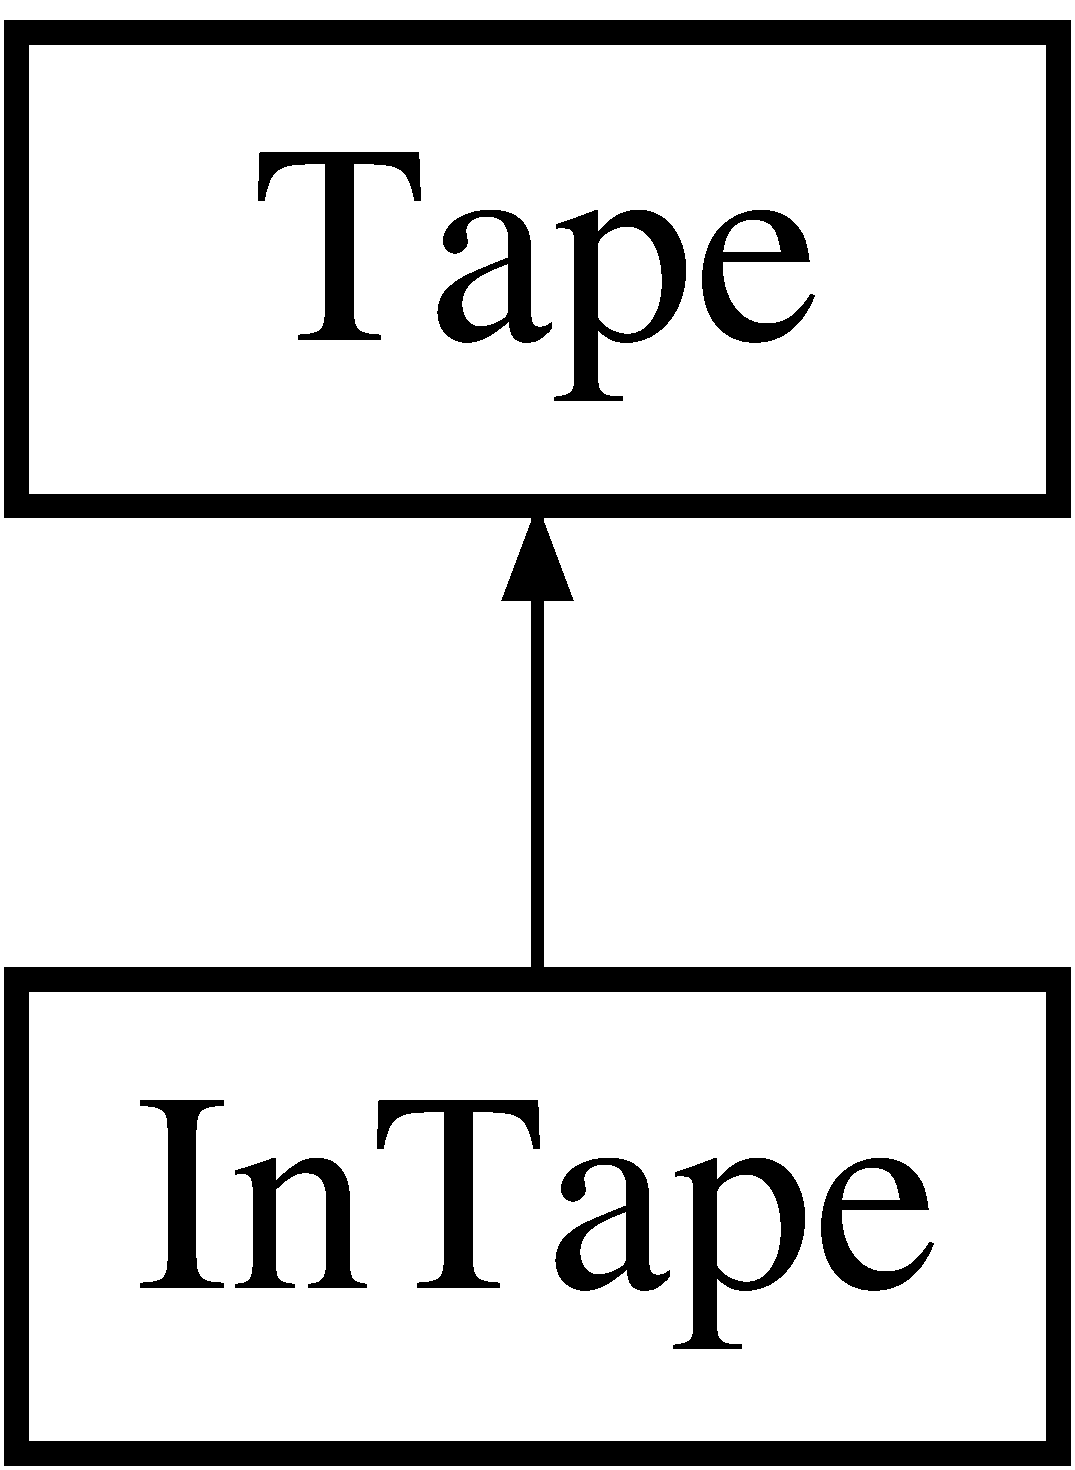
\includegraphics[height=2.000000cm]{classInTape}
\end{center}
\end{figure}
\subsection*{Public Member Functions}
\begin{DoxyCompactItemize}
\item 
\hypertarget{classInTape_a814ac605f20d11e3ce900c17b9676fb9}{{\bfseries In\-Tape} (string)}\label{classInTape_a814ac605f20d11e3ce900c17b9676fb9}

\item 
\hypertarget{classInTape_a3aab7f78892c5f6d18652dbf6d49a571}{t\-\_\-tape\-\_\-field\-\_\-value {\bfseries read} ()}\label{classInTape_a3aab7f78892c5f6d18652dbf6d49a571}

\item 
\hypertarget{classInTape_a37c277211ba120801b8cfeb9d3216dc4}{void {\bfseries reset} ()}\label{classInTape_a37c277211ba120801b8cfeb9d3216dc4}

\item 
\hypertarget{classInTape_a1521797ba73ba4ad89021e34db0f44e1}{void {\bfseries read\-From\-File} ()}\label{classInTape_a1521797ba73ba4ad89021e34db0f44e1}

\end{DoxyCompactItemize}
\subsection*{Additional Inherited Members}


The documentation for this class was generated from the following files\-:\begin{DoxyCompactItemize}
\item 
src/headers/In\-Tape.\-hpp\item 
src/In\-Tape.\-cpp\end{DoxyCompactItemize}

\hypertarget{classMemory}{\section{Memory Class Reference}
\label{classMemory}\index{Memory@{Memory}}
}
\subsection*{Public Member Functions}
\begin{DoxyCompactItemize}
\item 
\hypertarget{classMemory_a0a24b1f1fd76065f5c8b698d5b3eb8e0}{t\-\_\-register\-\_\-value {\bfseries read} (int)}\label{classMemory_a0a24b1f1fd76065f5c8b698d5b3eb8e0}

\item 
\hypertarget{classMemory_af7a465a9cb00fc8fb309949bfa0fa135}{t\-\_\-register\-\_\-value {\bfseries read\-Accum} ()}\label{classMemory_af7a465a9cb00fc8fb309949bfa0fa135}

\item 
\hypertarget{classMemory_ab5d352ec0e45e8507a30e807e23e593f}{void {\bfseries write} (t\-\_\-register\-\_\-value, int)}\label{classMemory_ab5d352ec0e45e8507a30e807e23e593f}

\item 
\hypertarget{classMemory_aea8f97249d2188cd8ee74147f7c73012}{void {\bfseries write\-Accum} (t\-\_\-register\-\_\-value)}\label{classMemory_aea8f97249d2188cd8ee74147f7c73012}

\item 
\hypertarget{classMemory_a4b6f224f9e77da560d18b517bcaaafc4}{void {\bfseries print} ()}\label{classMemory_a4b6f224f9e77da560d18b517bcaaafc4}

\item 
\hypertarget{classMemory_a2d53c704906468fb5dedf8e3649fb7b3}{void {\bfseries reset} ()}\label{classMemory_a2d53c704906468fb5dedf8e3649fb7b3}

\end{DoxyCompactItemize}


The documentation for this class was generated from the following files\-:\begin{DoxyCompactItemize}
\item 
src/headers/Memory.\-hpp\item 
src/Memory.\-cpp\end{DoxyCompactItemize}

\hypertarget{classOutTape}{\section{Out\-Tape Class Reference}
\label{classOutTape}\index{Out\-Tape@{Out\-Tape}}
}
Inheritance diagram for Out\-Tape\-:\begin{figure}[H]
\begin{center}
\leavevmode
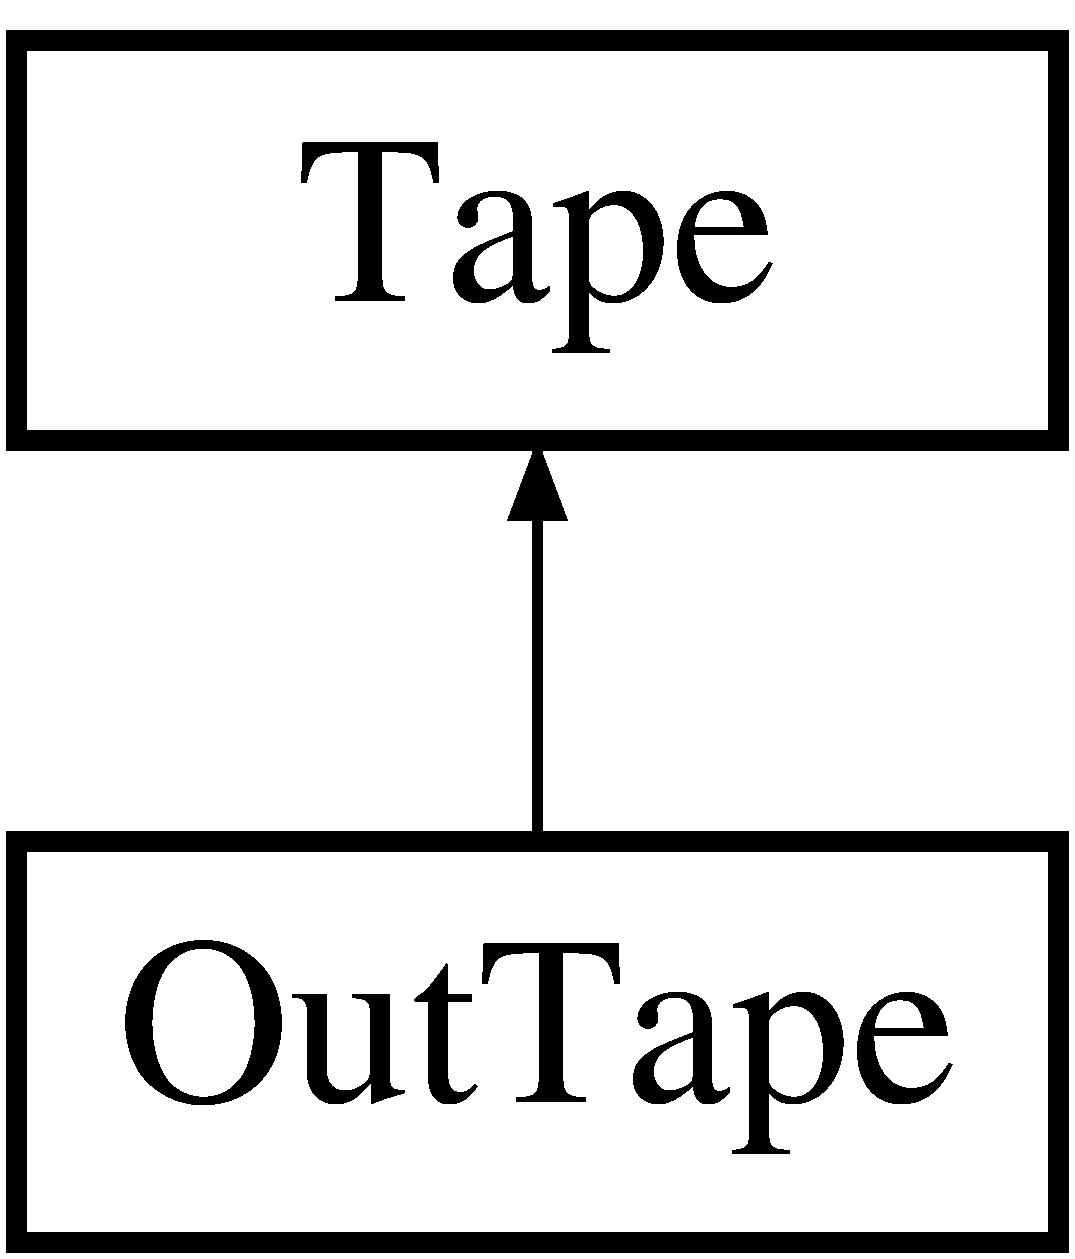
\includegraphics[height=2.000000cm]{classOutTape}
\end{center}
\end{figure}
\subsection*{Public Member Functions}
\begin{DoxyCompactItemize}
\item 
\hypertarget{classOutTape_aa2bcb3f0d40f7d9a0c562da036b89f34}{{\bfseries Out\-Tape} (string)}\label{classOutTape_aa2bcb3f0d40f7d9a0c562da036b89f34}

\item 
\hypertarget{classOutTape_ac88246c501c7725504842521a1e1aa79}{void {\bfseries write} (t\-\_\-tape\-\_\-field\-\_\-value)}\label{classOutTape_ac88246c501c7725504842521a1e1aa79}

\item 
\hypertarget{classOutTape_a7b217ae81e2caf28d9bad4b3ce3df8de}{void {\bfseries reset} ()}\label{classOutTape_a7b217ae81e2caf28d9bad4b3ce3df8de}

\item 
\hypertarget{classOutTape_a169b25fcd07a5abb4336940ff5d789fb}{void {\bfseries write\-On\-File} ()}\label{classOutTape_a169b25fcd07a5abb4336940ff5d789fb}

\end{DoxyCompactItemize}
\subsection*{Additional Inherited Members}


The documentation for this class was generated from the following files\-:\begin{DoxyCompactItemize}
\item 
src/headers/Out\-Tape.\-hpp\item 
src/Out\-Tape.\-cpp\end{DoxyCompactItemize}

\hypertarget{classPC}{\section{P\-C Class Reference}
\label{classPC}\index{P\-C@{P\-C}}
}
\subsection*{Public Member Functions}
\begin{DoxyCompactItemize}
\item 
\hypertarget{classPC_a4e974c3154857ffeab9112b99345ad60}{\hyperlink{classInstruction}{t\-\_\-instruction} {\bfseries get\-P\-Cinstruction} ()}\label{classPC_a4e974c3154857ffeab9112b99345ad60}

\item 
\hypertarget{classPC_a85d34e54abd197248883940c04d5570d}{void {\bfseries set\-P\-Cinstruction} (\hyperlink{classInstruction}{t\-\_\-instruction})}\label{classPC_a85d34e54abd197248883940c04d5570d}

\item 
\hypertarget{classPC_a3eb80177254d0cd8d4fd8c8ef68adaff}{t\-\_\-line {\bfseries get\-Current\-Line} ()}\label{classPC_a3eb80177254d0cd8d4fd8c8ef68adaff}

\item 
\hypertarget{classPC_a451dc96b1029b99e17797bb33529027b}{void {\bfseries set\-Current\-Line} (t\-\_\-line)}\label{classPC_a451dc96b1029b99e17797bb33529027b}

\end{DoxyCompactItemize}


The documentation for this class was generated from the following files\-:\begin{DoxyCompactItemize}
\item 
src/headers/P\-C.\-hpp\item 
src/P\-C.\-cpp\end{DoxyCompactItemize}

\hypertarget{classProgram}{\section{Program Class Reference}
\label{classProgram}\index{Program@{Program}}
}
\subsection*{Public Member Functions}
\begin{DoxyCompactItemize}
\item 
\hypertarget{classProgram_af6ada385f5b85e9b05d4ca77b1c662e2}{{\bfseries Program} (string)}\label{classProgram_af6ada385f5b85e9b05d4ca77b1c662e2}

\item 
\hypertarget{classProgram_abf7fd11e802491c2f4c30a907cdd04b1}{bool {\bfseries load\-Program\-From\-File} ()}\label{classProgram_abf7fd11e802491c2f4c30a907cdd04b1}

\item 
\hypertarget{classProgram_a8856fb9ed6c88db42b690ab0f80f2eaf}{void {\bfseries show\-Program} ()}\label{classProgram_a8856fb9ed6c88db42b690ab0f80f2eaf}

\item 
\hypertarget{classProgram_ab055b0a34e04fa8bd459e5d6ab4e124a}{bool {\bfseries exist\-Tag} (\hyperlink{classTag}{Tag})}\label{classProgram_ab055b0a34e04fa8bd459e5d6ab4e124a}

\item 
\hypertarget{classProgram_aa4118e50ec51f80f60b392024d192908}{bool {\bfseries exist\-Tag} (string)}\label{classProgram_aa4118e50ec51f80f60b392024d192908}

\item 
\hypertarget{classProgram_ab0dc75a521028081adc9aeb9fb2f2d01}{void {\bfseries move\-To\-Next\-Instruction} ()}\label{classProgram_ab0dc75a521028081adc9aeb9fb2f2d01}

\item 
\hypertarget{classProgram_a5f00f8b1075c97456d2b1d3c30fad7f3}{void {\bfseries set\-Next\-Instruction} (\hyperlink{classInstruction}{Instruction}, int)}\label{classProgram_a5f00f8b1075c97456d2b1d3c30fad7f3}

\item 
\hypertarget{classProgram_a0198da3741cd6bfe090d10f39f437924}{t\-\_\-program {\bfseries get\-Program} ()}\label{classProgram_a0198da3741cd6bfe090d10f39f437924}

\item 
\hypertarget{classProgram_a7814e3bdc4d91b57205109b964a51cbd}{t\-\_\-tags {\bfseries get\-Tags} ()}\label{classProgram_a7814e3bdc4d91b57205109b964a51cbd}

\item 
\hypertarget{classProgram_a7f77cefd84d0a9f31bc2909af70980bf}{\hyperlink{classPC}{P\-C} {\bfseries get\-P\-C} ()}\label{classProgram_a7f77cefd84d0a9f31bc2909af70980bf}

\item 
\hypertarget{classProgram_a2397451fffeeca19728ebbf2ea68f26b}{void {\bfseries reload} (string)}\label{classProgram_a2397451fffeeca19728ebbf2ea68f26b}

\item 
\hypertarget{classProgram_aeb6d22c6dc2202ea374fc6b9ce81a2f4}{void {\bfseries reset} ()}\label{classProgram_aeb6d22c6dc2202ea374fc6b9ce81a2f4}

\item 
\hypertarget{classProgram_a8cb065b057057bb900d290b1df63563f}{void {\bfseries init\-P\-C} ()}\label{classProgram_a8cb065b057057bb900d290b1df63563f}

\item 
\hypertarget{classProgram_af1e2b12f80a13528c39692d9ee1a7bcb}{string {\bfseries get\-File} ()}\label{classProgram_af1e2b12f80a13528c39692d9ee1a7bcb}

\end{DoxyCompactItemize}


The documentation for this class was generated from the following files\-:\begin{DoxyCompactItemize}
\item 
src/headers/Program.\-hpp\item 
src/Program.\-cpp\end{DoxyCompactItemize}

\hypertarget{classRAMmachine}{\section{R\-A\-Mmachine Class Reference}
\label{classRAMmachine}\index{R\-A\-Mmachine@{R\-A\-Mmachine}}
}
\subsection*{Public Member Functions}
\begin{DoxyCompactItemize}
\item 
\hypertarget{classRAMmachine_ad5ec54172e71b87c76f8a4b4d31e06bd}{{\bfseries R\-A\-Mmachine} (string, string, string)}\label{classRAMmachine_ad5ec54172e71b87c76f8a4b4d31e06bd}

\item 
\hypertarget{classRAMmachine_a42b4e5cc1c054c28011e00ab54c98bbf}{void {\bfseries init\-Machine} (string, string, string)}\label{classRAMmachine_a42b4e5cc1c054c28011e00ab54c98bbf}

\item 
\hypertarget{classRAMmachine_a4e5efa9b417958cd42f649f66e237710}{void {\bfseries run} (bool)}\label{classRAMmachine_a4e5efa9b417958cd42f649f66e237710}

\item 
\hypertarget{classRAMmachine_ade5769f9ae186bed299fa164d16ebc33}{void {\bfseries print\-Current\-Instruction} ()}\label{classRAMmachine_ade5769f9ae186bed299fa164d16ebc33}

\item 
\hypertarget{classRAMmachine_a94145ee5533985c15c38156069a7b67e}{void {\bfseries show\-Memory\-Status} ()}\label{classRAMmachine_a94145ee5533985c15c38156069a7b67e}

\item 
\hypertarget{classRAMmachine_a9d0a4de83f7bb48565f7abb370215ac0}{void {\bfseries show\-Program} ()}\label{classRAMmachine_a9d0a4de83f7bb48565f7abb370215ac0}

\item 
\hypertarget{classRAMmachine_ada124c82636c272ef71f82e5dec53a41}{void {\bfseries print\-Input\-Tape} ()}\label{classRAMmachine_ada124c82636c272ef71f82e5dec53a41}

\item 
\hypertarget{classRAMmachine_ac8fe4966b254a0663685d5d42521814c}{void {\bfseries print\-Output\-Tape} ()}\label{classRAMmachine_ac8fe4966b254a0663685d5d42521814c}

\item 
\hypertarget{classRAMmachine_a5b1d7da020547c622f787e3d831ddda8}{void {\bfseries wait\-For\-Key} ()}\label{classRAMmachine_a5b1d7da020547c622f787e3d831ddda8}

\item 
\hypertarget{classRAMmachine_a9ec0b4a2dac71d87bdfa662d1e0a11d6}{\hyperlink{classProgram}{Program} {\bfseries get\-Program} ()}\label{classRAMmachine_a9ec0b4a2dac71d87bdfa662d1e0a11d6}

\item 
\hypertarget{classRAMmachine_ab366057d4a54d9d0acd2b7a89612af9a}{\hyperlink{classInTape}{In\-Tape} {\bfseries get\-Input\-Tape} ()}\label{classRAMmachine_ab366057d4a54d9d0acd2b7a89612af9a}

\item 
\hypertarget{classRAMmachine_a6a2999d602c5c88391c4dc4e39916c1d}{\hyperlink{classOutTape}{Out\-Tape} {\bfseries get\-Output\-Tape} ()}\label{classRAMmachine_a6a2999d602c5c88391c4dc4e39916c1d}

\item 
\hypertarget{classRAMmachine_ac28a9d66c715f606a3cf30259edbf115}{void {\bfseries set\-Program} (\hyperlink{classProgram}{Program} prog)}\label{classRAMmachine_ac28a9d66c715f606a3cf30259edbf115}

\end{DoxyCompactItemize}


The documentation for this class was generated from the following files\-:\begin{DoxyCompactItemize}
\item 
src/headers/R\-A\-Mmachine.\-hpp\item 
src/R\-A\-Mmachine.\-cpp\end{DoxyCompactItemize}

\hypertarget{classRegister}{\section{Register Class Reference}
\label{classRegister}\index{Register@{Register}}
}
\subsection*{Public Member Functions}
\begin{DoxyCompactItemize}
\item 
\hypertarget{classRegister_aaf6b622206afd2e9646a6da08c68e958}{{\bfseries Register} (t\-\_\-register\-\_\-value)}\label{classRegister_aaf6b622206afd2e9646a6da08c68e958}

\item 
\hypertarget{classRegister_a01d391e6f2251d6aae7176c4c1c05a0c}{void {\bfseries set\-\_\-value} (t\-\_\-register\-\_\-value)}\label{classRegister_a01d391e6f2251d6aae7176c4c1c05a0c}

\item 
\hypertarget{classRegister_a1c1996453221cc2536466887e891992d}{t\-\_\-register\-\_\-value {\bfseries get\-\_\-value} ()}\label{classRegister_a1c1996453221cc2536466887e891992d}

\item 
\hypertarget{classRegister_a4a354186661756dee96799db1219a20a}{void {\bfseries reset} ()}\label{classRegister_a4a354186661756dee96799db1219a20a}

\item 
\hypertarget{classRegister_a8e738fe7c0bb54be62bf084abf347e7d}{void {\bfseries print} ()}\label{classRegister_a8e738fe7c0bb54be62bf084abf347e7d}

\end{DoxyCompactItemize}


The documentation for this class was generated from the following files\-:\begin{DoxyCompactItemize}
\item 
src/headers/Register.\-hpp\item 
src/Register.\-cpp\end{DoxyCompactItemize}

\hypertarget{classTag}{\section{Tag Class Reference}
\label{classTag}\index{Tag@{Tag}}
}
\subsection*{Public Member Functions}
\begin{DoxyCompactItemize}
\item 
\hypertarget{classTag_a8c107d520a979dccc728bf72e3bdc344}{{\bfseries Tag} (string, t\-\_\-line\-\_\-number, t\-\_\-pos\-\_\-number)}\label{classTag_a8c107d520a979dccc728bf72e3bdc344}

\item 
\hypertarget{classTag_aad68995f5e8193da6e8faf8b9612f25a}{string {\bfseries get\-\_\-tag\-\_\-identifier} ()}\label{classTag_aad68995f5e8193da6e8faf8b9612f25a}

\item 
\hypertarget{classTag_a0c37771e42b042ae25366bd3108fe9d3}{t\-\_\-line\-\_\-number {\bfseries get\-\_\-line\-\_\-number} ()}\label{classTag_a0c37771e42b042ae25366bd3108fe9d3}

\item 
\hypertarget{classTag_a3135714a611ab1ef50461e9989fb430c}{string {\bfseries get\-\_\-saved\-\_\-number\-\_\-pos} ()}\label{classTag_a3135714a611ab1ef50461e9989fb430c}

\item 
\hypertarget{classTag_ad91d8073141dde83849df8fe24ce8f46}{bool {\bfseries operator==} (\hyperlink{classTag}{Tag} \&)}\label{classTag_ad91d8073141dde83849df8fe24ce8f46}

\end{DoxyCompactItemize}


The documentation for this class was generated from the following files\-:\begin{DoxyCompactItemize}
\item 
src/headers/Tag.\-hpp\item 
src/Tag.\-cpp\end{DoxyCompactItemize}

\hypertarget{classTape}{\section{Tape Class Reference}
\label{classTape}\index{Tape@{Tape}}
}
Inheritance diagram for Tape\-:\begin{figure}[H]
\begin{center}
\leavevmode
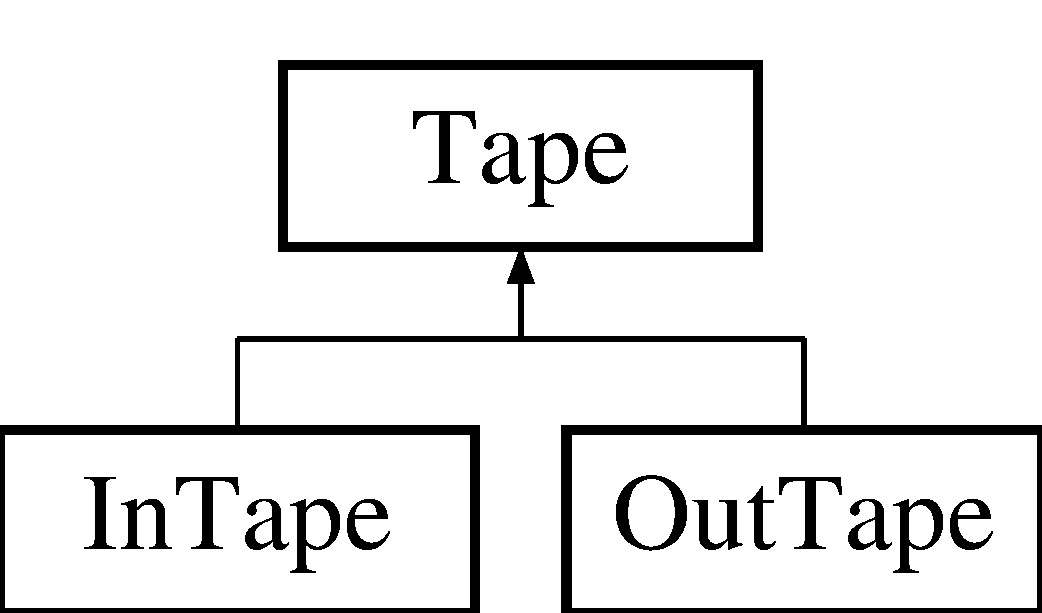
\includegraphics[height=2.000000cm]{classTape}
\end{center}
\end{figure}
\subsection*{Public Member Functions}
\begin{DoxyCompactItemize}
\item 
\hypertarget{classTape_a5f06dea26c7e30c323613f52b5edea62}{virtual void {\bfseries reset} ()=0}\label{classTape_a5f06dea26c7e30c323613f52b5edea62}

\item 
\hypertarget{classTape_a90be518f537d4210cee05b716feede36}{int {\bfseries get\-Tape\-Size} ()}\label{classTape_a90be518f537d4210cee05b716feede36}

\item 
\hypertarget{classTape_a2906a5dbf3c52729b0ae5a336c3828b6}{void {\bfseries print} ()}\label{classTape_a2906a5dbf3c52729b0ae5a336c3828b6}

\end{DoxyCompactItemize}
\subsection*{Protected Member Functions}
\begin{DoxyCompactItemize}
\item 
\hypertarget{classTape_a0a6f4c9427e679f2ff77b4c0c2792429}{void {\bfseries set\-File} (string)}\label{classTape_a0a6f4c9427e679f2ff77b4c0c2792429}

\item 
\hypertarget{classTape_ac57754a7bdde56b9509a9a992b833e97}{string {\bfseries get\-File} ()}\label{classTape_ac57754a7bdde56b9509a9a992b833e97}

\end{DoxyCompactItemize}
\subsection*{Protected Attributes}
\begin{DoxyCompactItemize}
\item 
\hypertarget{classTape_af86585d00cfbcf8e14d4188f0ae4ec25}{t\-\_\-tape {\bfseries tape\-\_\-}}\label{classTape_af86585d00cfbcf8e14d4188f0ae4ec25}

\item 
\hypertarget{classTape_aed2ca258c7ab970769e97fa6b9ef4c6e}{string {\bfseries filename\-\_\-}}\label{classTape_aed2ca258c7ab970769e97fa6b9ef4c6e}

\end{DoxyCompactItemize}


The documentation for this class was generated from the following files\-:\begin{DoxyCompactItemize}
\item 
src/headers/Tape.\-hpp\item 
src/Tape.\-cpp\end{DoxyCompactItemize}

%--- End generated contents ---

% Index
\newpage
\phantomsection
\addcontentsline{toc}{chapter}{Index}
\printindex

\end{document}
